\section{Popis paralelního algoritmu a jeho implementace v OpenMP -- taskový paralelismus}

Prvním krokem pro paralelizaci bylo použít knihovnu OpenMP, a to konkrétně \textbf{taskový paralelismus}. Ten je v~OpenMP velmi jednoduchý na implementaci, jelikož stačilo v podstatě pouze přidat direktivu preprocesoru \mintinline{c}{#pragma omp task if(state.matrixPos < state.matrixLen / TASK_LEN)} ke každému rekurzivními volání funkce \mintinline{c}{weight_inner}, přidat aktualizaci globální proměnné nejlepšího stavu do \mintinline{c}{#pragma omp critical} a zaobalit první volání funkce do paralelního regionu s \mintinline{c}{#pragma omp single}, aby se DFS nepustilo na každém vlákně.

OpenMP pak na prvním vlákně spustí první \mintinline{c}{weight_inner}, a při každém dalším volání vytvoří nový \textbf{task}, který přidá do task poolu a distribuuje jednotlivým vláknům. Aby \textbf{nedocházelo} k vytváření velkého množství tasků, které by pak kvůli režii synchronizaci mezi vlákny \textbf{zpomalilo} program, používám podmínku, že task se spustí pouze tehdy, pokud je pozice v matici v první \mintinline{c}{1 / TASK_LEN}-tině. Jako nejvhodnější konstanta \mintinline{c}{TASK_LEN} se mi po spuštění několika běhů na několika instancích osvědčila $25$.

\section{Popis paralelního algoritmu a jeho implementace v OpenMP -- datový paralelismus}

Implementace v OpenMP pomocí \textbf{datového paralelismu} již byla o něco složitější. Nejprve jsem změnil \textbf{wrapper} funkci \mintinline{c}{weight}, která v taskovém paralelismu pouze zavolala \mintinline{c}{weight_inner} a to tak, aby s pomocí BFS vygenerovala 2 $\cdot$ počet vláken stavů. Pro to jsem vytvořil lehce upravenou funkci \mintinline{c}{weight_inner_bfs}, která má úplně stejnou implementaci, jako \mintinline{c}{weight_inner} s tím rozdílem, že místo rekurzivního volání sebe sama přidává nově vzniklý stav do \textbf{fronty}. Tato funkce se volá tak dlouho, dokud není dosažen potřebný počet stavů.

Jakmile je vygenerován dostatečný počet stavů, s pomocí direktivy \mintinline{c}{#pragma omp parallel for} jednotlivé stavy distribuuji mezi jednotlivá vlákna, na které zavolám původní rekurzivní funkci \mintinline{c}{weight_inner} (přejmenovanou na \mintinline{c}{weight_seq_rec}), která oproti sekvenčnímu řešení akorát používá ono \mintinline{c}{#pragma omp critical}.

Stejně jako sekvenční program, tak i oba dva paralelní programy (taskový i datový paralelismus) jsem spustil na školním počítači. Na ukázkových datech z Courses byly programy ještě \textbf{pomalejší}, jelikož byla tato data tak malá a jednoduchá, že režie \textbf{převážila} ono paralelní zrychlení. Na složitějších instancích již bylo zrychlení znát a jako \textbf{efektivnější} se ukázal \textbf{datový} paralelismus -- především díky tomu, že pomocí BFS rozdělí stavový prostor rovnoměrněji mezi jednotlivá vlákna než taskový pomocí DFS.

Pokud se podíváme na \textbf{graf zrychlení}, je zajímavé, že zatímco zrychlení u taskového paralelismu je (na 8 vláknech) \textbf{stabilně} mezi 2-3x, zrychlení u datového paralelismu je většinou okolo 5x, ale na některých instancích \textbf{spadne} na 2,5 -- na některých instancích bude tedy graf stavového prostoru značně nevyvážený \textit{(jedno vlákno pak počítá v situaci, kdy už ostatní dopracovala)}.

\begin{figure}[H]
    \centering
    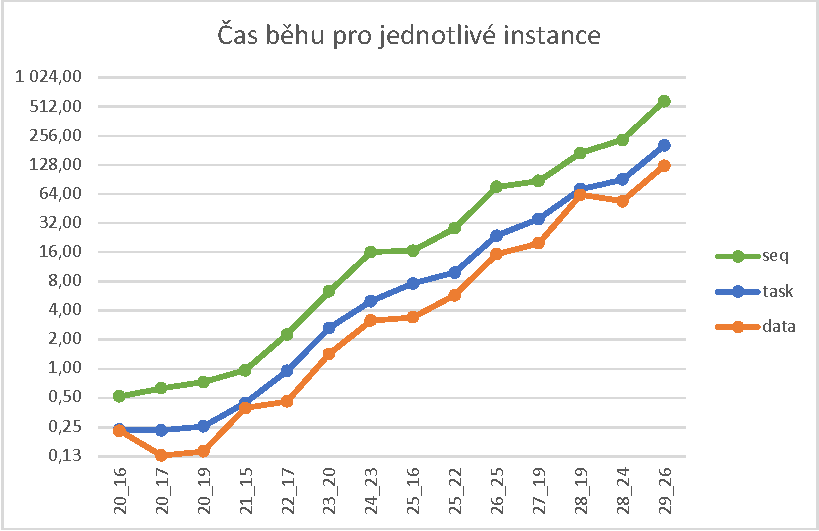
\includegraphics[width=0.45\textwidth]{fig/2_1.pdf}
    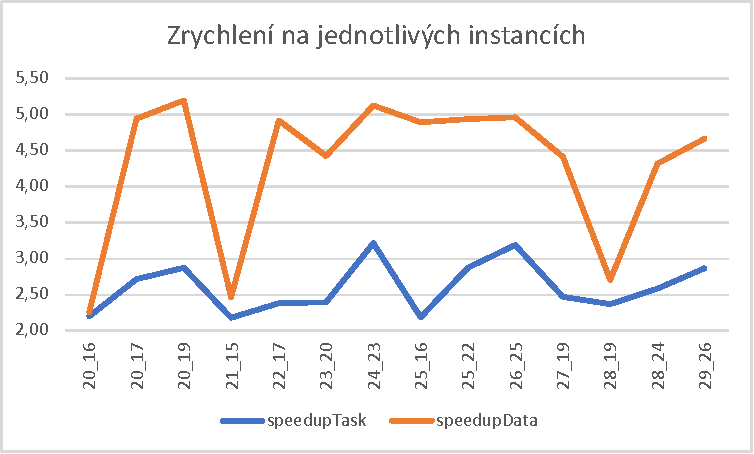
\includegraphics[width=0.485\textwidth]{fig/2_2.pdf}
    \caption{Časy běhu a zrychlení na jednotlivých instancích}
\end{figure}
